\chapter{Datasets, Simulated Samples and Triggers}
\label{chap:Samples}

This analysis is based on data collected by the \ac{CMS} experiment in 2016-2018 from $pp$ collisions at a center-of-mass energy of 13 TeV corresponding to an integrated luminosity of 138 fb$^{-1}$. There were approximately 30 simultaneous $pp$ collisions occurring per 25 ns. Based on online selection criteria, fully reconstructed collision data that contain high-level physics objects are divided in ``\acp{PD}'', which include ``DoubleEG'', ``DoubleMu'', ``MuonEG'', ``SingleElectron'', and ``SingleMuon'' for 2016 and 2017 data taking era. In 2018, ``SingleElectron'', ``DoubleEG'' are replaced by ``EGamma''. The names of these \acp{PD} reflect the selection criteria. The data taking conditions in 2016-2018 were difference across the years. To account for this, all \ac{MC} samples are generated separately for each year separately. 
%%%%%%%%%%%%%%%%%%%%%%%%%%%%%%%%%%%%%%%%%%%%%%%%%%%%%%%%%%%%%
%%%%%%%%%%%%%%%%%%%%%%%%%%%%%%%%%%%%%%%%%%%%%%%%%%%%%%%%%%%%%
\section{Signal Samples}
\label{sec:Signals}

\begin{table}[t]
\sffamily
\centering
\caption{Summary of relevant dimension-6 operators considered in this analysis. Here, $\varepsilon$ is the two dimensional Levi-Civita symbol, $\gamma^\mu$ the gamma matrix, and $\sigma^{\mu\nu}=\frac{\textsf{i}}{2}[\gamma^\mu,\gamma^\nu]$. The l and q denote left-handed doublets, whereas u and e denote right-handed singlets. The indices $i$ and $j$ are lepton flavor indices that run from 1 to 2 with $i \neq j$; $m$ and $n$ are quark flavor indices with the condition that one of them is 3 and the other one is 1 or 2.}
\begin{tabular}{cccl}
\toprule
Lorentz Structure & \multicolumn{3}{c}{Operator}\\
\midrule
\multirow{4}{*}{vector} & $\textsf{O}_{\textsf{lq}}^{(1)ijmn}$ &=& $(\overline{\textsf{l}}_i\gamma^\mu\textsf{l}_j)
   (\overline{\textsf{q}}_m\gamma_\mu\textsf{q}_n)$
   \\
  & $\textsf{O}_{\textsf{lu}}^{ijmn}$ &=& $(\overline{\textsf{l}}_i\gamma^\mu\textsf{l}_j)
   (\overline{\textsf{u}}_m\gamma_\mu\textsf{u}_n)$
   \\  
  & $\textsf{O}_{\textsf{eq}}^{ijmn}$ &=& $(\overline{\textsf{e}}_i\gamma^\mu\textsf{e}_j)
   (\overline{\textsf{q}}_m\gamma_\mu\textsf{q}_n)$
   \\ 
  & $\textsf{O}_{\textsf{eu}}^{ijmn}$ &=& $(\overline{\textsf{e}}_i\gamma^\mu\textsf{e}_j)
   (\overline{\textsf{u}}_m\gamma_\mu\textsf{u}_n)$
   \\ \midrule
\multirow{1}{*}{scalar}  & $\textsf{O}_{\textsf{lequ}}^{(1)ijmn}$ &=& $(\overline{\textsf{l}}_i\textsf{e}_j)\;\varepsilon\;
   (\overline{\textsf{q}}_m\textsf{u}_n)$
   \\ 
 \multirow{1}{*}{tensor} & $\textsf{O}_{\textsf{lequ}}^{(3)ijmn}$ &=& $(\overline{\textsf{l}}_i \sigma^{\mu\nu}\textsf{e}_j)\;\varepsilon\;
   (\overline{\textsf{q}}_m\sigma_{\mu\nu}\textsf{u}_n)$
  \\ \bottomrule
\end{tabular}
\label{tab:dimension6}
\end{table}

In this analysis, New Physics  is described by Dimension-6 \ac{EFT} operators,

\begin{equation}
\label{eq:0}
\mathcal{L}=\mathcal{L}_{\text{SM}}^{(4)} + \frac{1}{\Lam^2}\sum_{a}\WC{(6)}{a}\OP{(6)}{a}+O\left( \frac{1}{\Lam^4}\right).
\end{equation}  

Among many of the Dimension-6 operators in Warsaw basis~\cite{Aguilar-Saavedra:2018ksv}, a total of 6 operators are considered, which are summarized in Table~\ref{tab:dimension6}. To reduce the number of free parameters, the permutations of fermion flavors are combined. Taking $\emut{u}$ vertex as an example, the \acp{WC} are parameterized in the following way:

\begin{eqnarray}
\label{eq:1:0}
 \textsf{C}_{\textsf{lq}}
 &=& \textsf{C}_{\textsf{lq}}^{(1)1213}
 + \textsf{C}_{\textsf{lq}}^{(1)2113}
 + \textsf{C}_{\textsf{lq}}^{(1)1231}
 + \textsf{C}_{\textsf{lq}}^{(1)1213}
 ,\\
\label{eq1:1}
 \textsf{C}_{\textsf{lu}}  
 &=& \textsf{C}_{\textsf{lu}}^{1213}
 + \textsf{C}_{\textsf{lu}}^{2113}
 + \textsf{C}_{\textsf{lu}}^{1231}
 + \textsf{C}_{\textsf{lu}}^{1213}
 ,\\ 
\label{eq:1:2}
 \textsf{C}_{\textsf{eq}}
 &=& \textsf{C}_{\textsf{eq}}^{1213}
 + \textsf{C}_{\textsf{eq}}^{2113}
 + \textsf{C}_{\textsf{eq}}^{1231}
 + \textsf{C}_{\textsf{eq}}^{1213}
 ,\\
\label{eq:1:3}
 \textsf{C}_{\textsf{eu}}  
 &=& \textsf{C}_{\textsf{eu}}^{1213}
 + \textsf{C}_{\textsf{eu}}^{2113}
 + \textsf{C}_{\textsf{eu}}^{1231}
 + \textsf{C}_{\textsf{eu}}^{1213}
 ,\\
\label{eq:1:4}
 \textsf{C}_{\textsf{lequ}}^{(1)}  
 &=& \textsf{C}_{\textsf{lequ}}^{(1)1213}
 + \textsf{C}_{\textsf{lequ}}^{(1)2113}
 + \textsf{C}_{\textsf{lequ}}^{(1)1231}
 + \textsf{C}_{\textsf{lequ}}^{(1)1213}
  ,\\
\label{eq:1:5}
 \textsf{C}_{\textsf{lequ}}^{(3)}
 &=& \textsf{C}_{\textsf{lequ}}^{(3)1213}
 + \textsf{C}_{\textsf{lequ}}^{(3)2113}
 + \textsf{C}_{\textsf{lequ}}^{(3)1231}
 + \textsf{C}_{\textsf{lequ}}^{(3)1213}. 
\end{eqnarray}

Additionally, all vector-like operators are combined,

\begin{eqnarray}
\label{eq:1:6}
 \OP{\textsf{vector}}{\emut{u}}&=&\OP{}{\textsf{lq}}+\OP{}{\textsf{lu}}+\OP{}{\textsf{eq}}+\OP{}{\textsf{eu}},\\
\label{eq:1:7}
 \OP{\textsf{scalar}}{\emut{u}}&=&\OP{(1)}{\textsf{lequ}}+\textsf{h.c},\\
\label{eq:1:8}
 \OP{\textsf{tensor}}{\emut{u}}&=&\OP{(3)}{\textsf{lequ}}+\textsf{h.c},
\end{eqnarray}

which results in 6 independent \acp{WC}: $\WC{\textsf{vector}}{\emut{u}},~\WC{\textsf{scalar}}{\emut{u}},~\WC{\textsf{tensor}}{\emut{u}},~\WC{\textsf{vector}}{\emut{c}},~\WC{\textsf{scalar}}{\emut{c}},~\WC{\textsf{tensor}}{\emut{c}}.$  

To generate signal \ac{MC} samples, the effective Lagrangian described above is implemented using the SmeftFR v2~\cite{Dedes:2019uzs} model, and saved in the ``UFO'' format~\cite{Degrande:2011ua}. Additionally, all the \acp{WC} are set to 1 with $\Lam$ = 1 TeV in the UFO, which then interfaces with the \textsc{FeynRules}~\cite{Christensen:2008py} package to calculate Feynman diagrams. The output of the \FR~is used in \ac{ME} generator \MG~v2.4.2~\cite{Alwall:2014hca} to generate events at the leading order.

\begin{figure}[tbh!]
 \begin{center}
 \begin{tabular}{cc}
  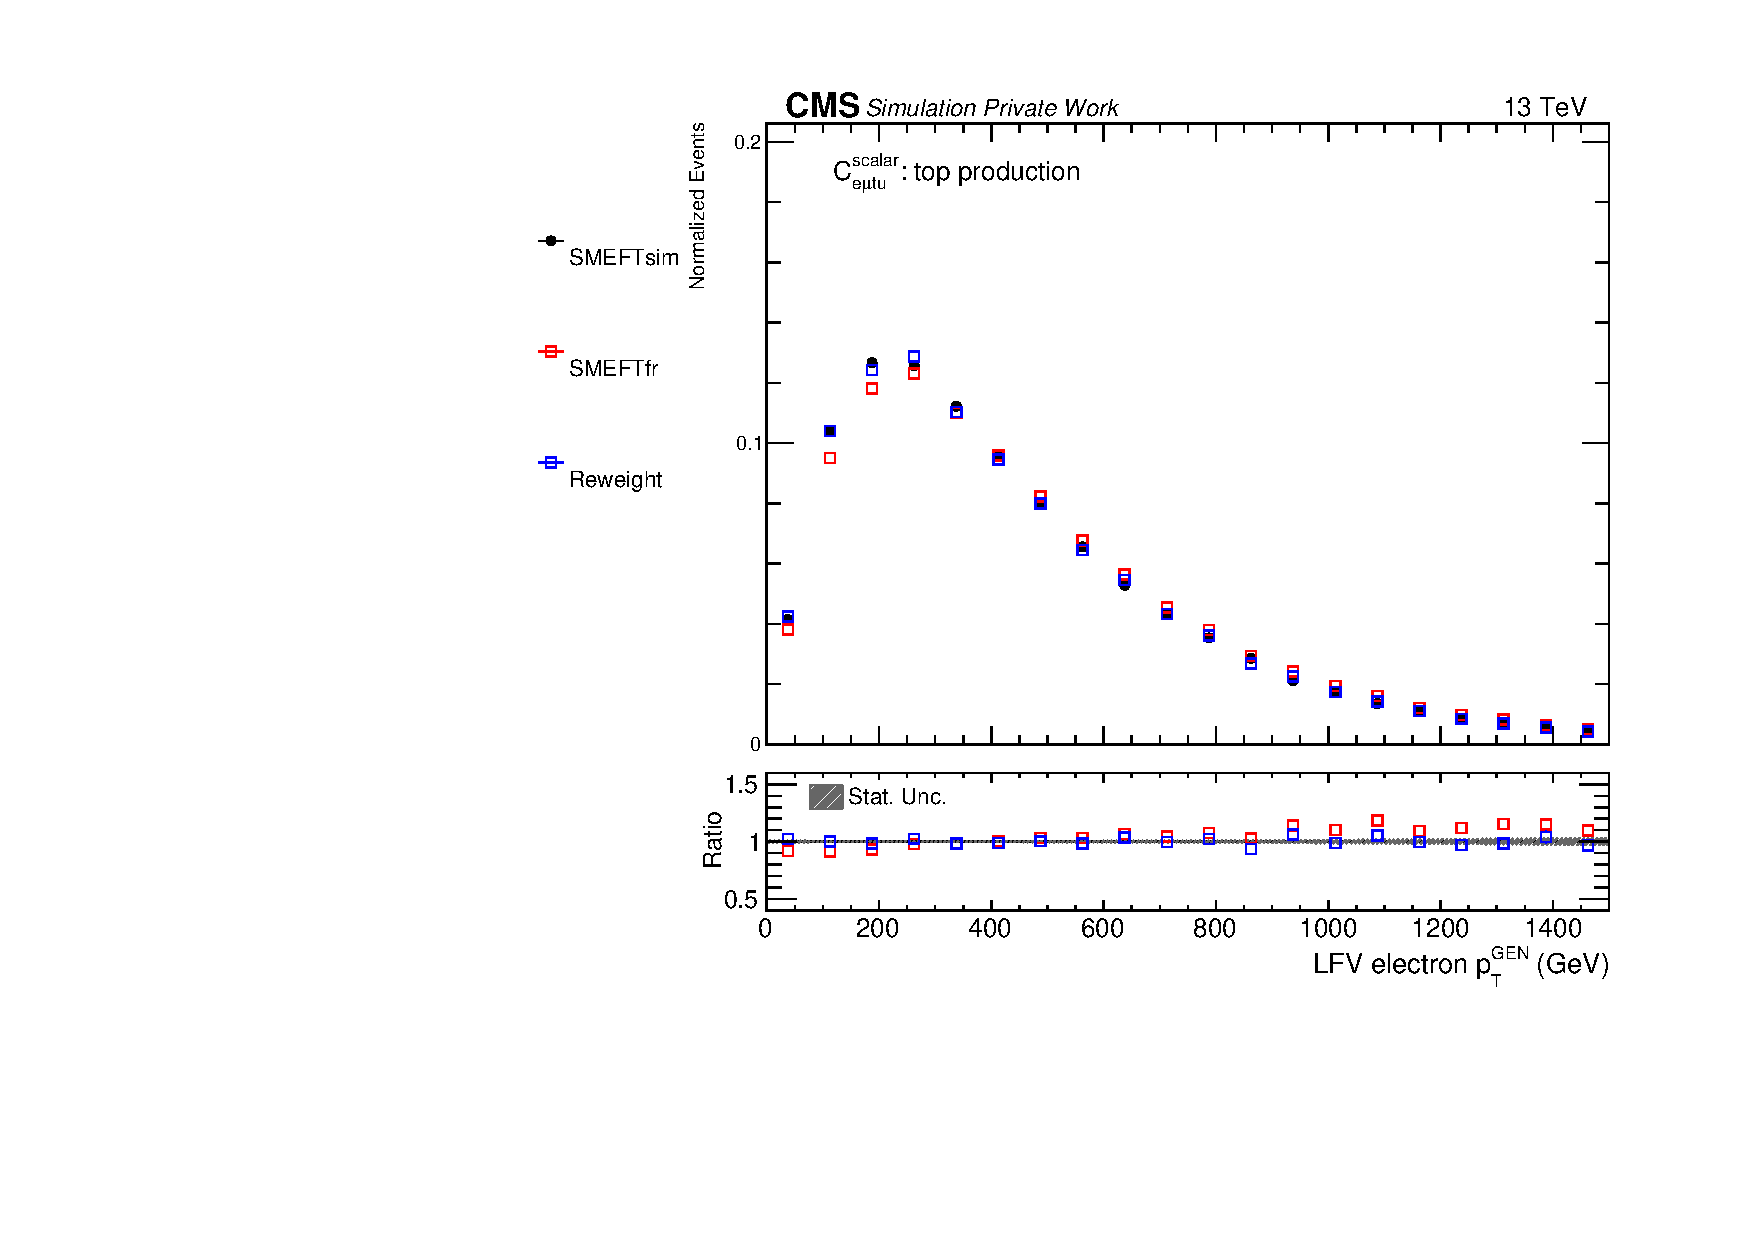
\includegraphics[width=0.48\textwidth]{figures/Part3/Samples/LFVePt}&
    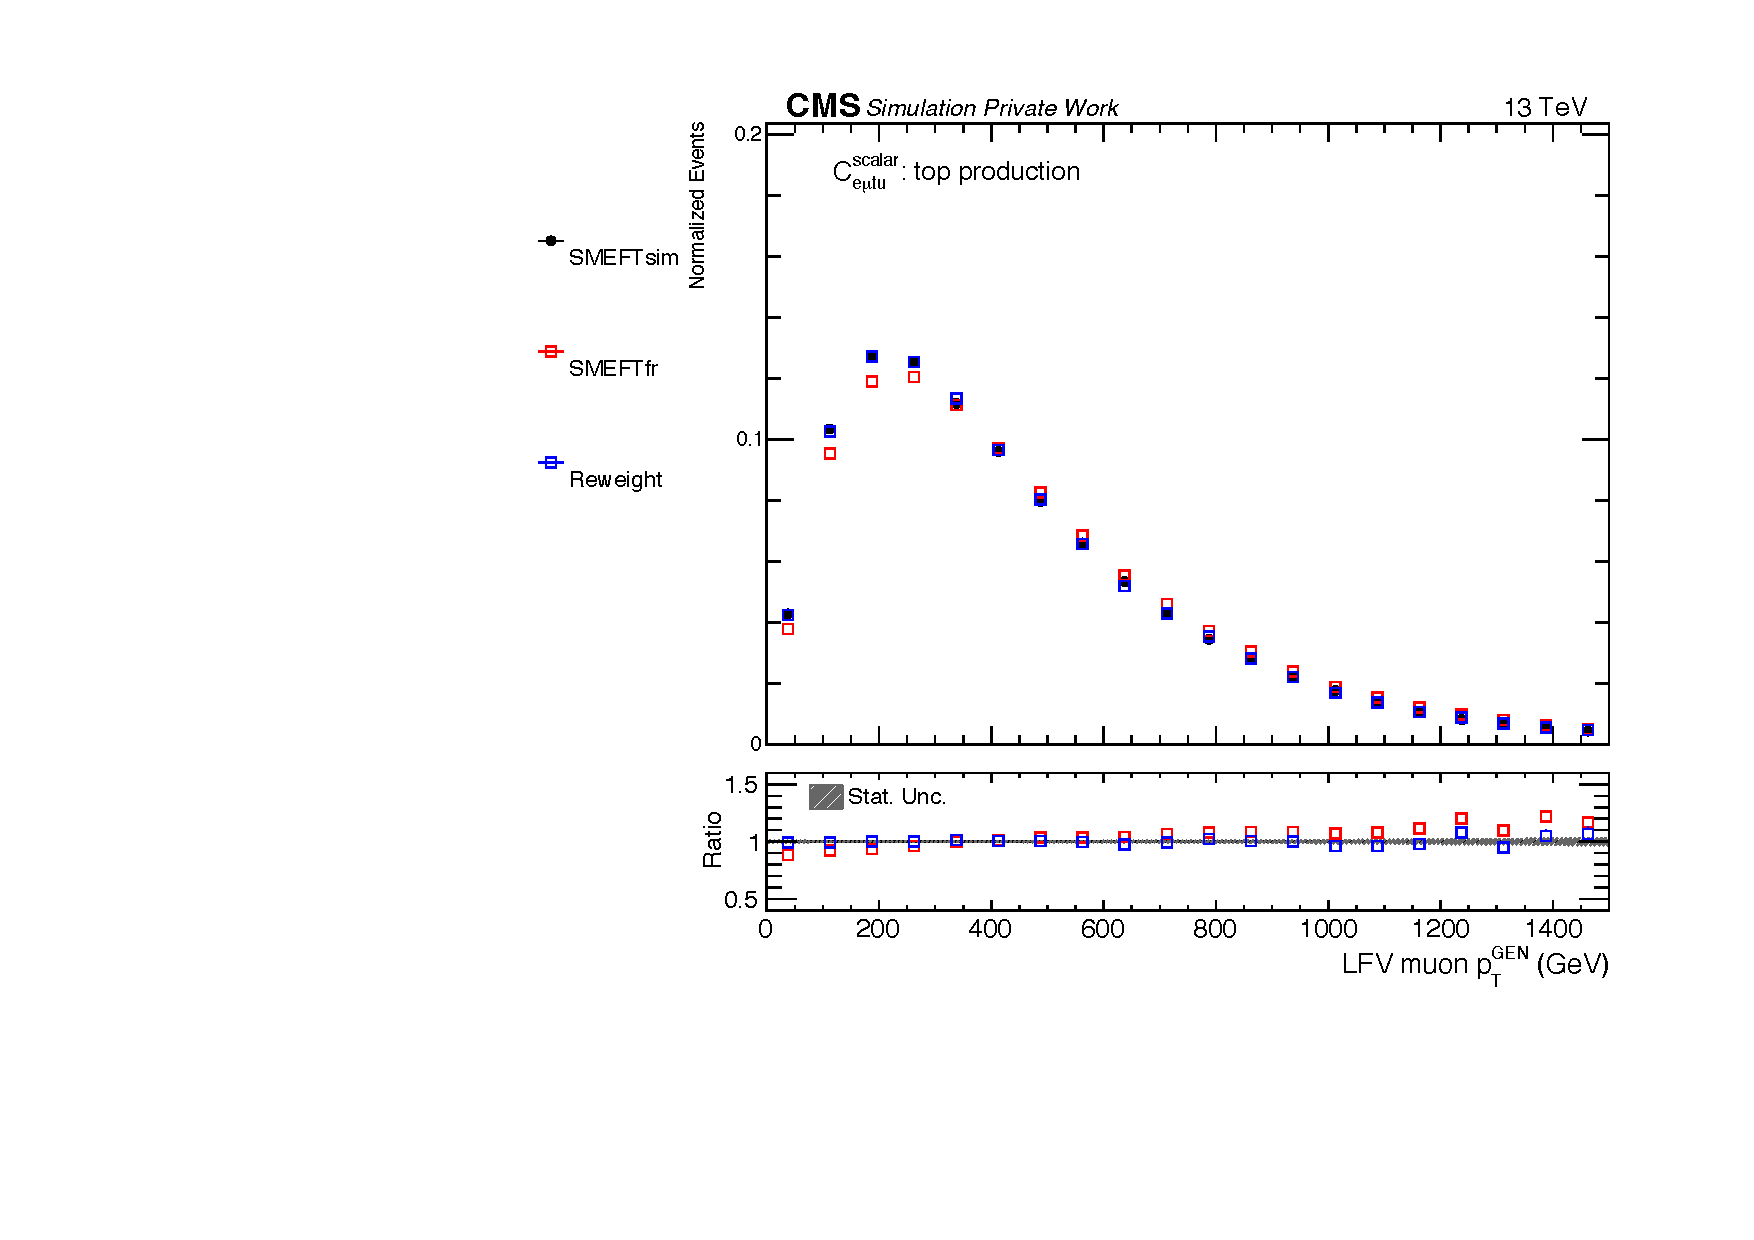
\includegraphics[width=0.48\textwidth]{figures/Part3/Samples/LFVmuPt}\\
 \end{tabular}
 \caption{Comparison of kinematic distributions at \ac{ME}-level produced by different models: LFV electron $\pt$ (left), LFV muon $\pt$ (right). The ``SmeftFR'' samples (shown in red curve) and  ``SMEFTsim'' samples (shown in black curve) are statistically independent of each other. The ``Reweight'' (shown in blue curve) are produced by applying weights calculated by Equation~\ref{eq:2} to ``SmeftFR'' samples.}
 \label{fig:reweight}
 \end{center}
\end{figure}

In general, the calculations done by the \ac{ME} generators are model-agnostic assuming the same \ac{EFT} configurations. In other words, models like SmeftFR or SMEFTsim~\cite{Brivio:2017btx} are expected to give the same or very similar results in terms of cross sections and four-momenta of final-state particles. Nevertheless, visible differences in kinematics have been observed and shown in Figure~\ref{fig:reweight}. Furthermore, the cross sections predicted by SmeftFR v2 also yield more than 20\% difference relative to SMEFTsim due to a bug that was later fixed in SmeftFR v3. In the light of these differences, the \ac{CMS} and \ac{ATLAS} Collaborations agreed to adopt the SMEFTsim model as the common standard.  To quantify the impact of the choice of models on kinematics, the following ratio is calculated for each event $i$,

\begin{equation}
\label{eq:2}
R_{\textsf{reweight}}^{i}=\frac{\omega_{\textsf{SMEFTsim}}^i}{\omega_{\textsf{SmeftFR}}^i},
\end{equation}

where $\omega^{i}_{X}$ is the per-event \ac{ME} weight calculated by \MG~using model $X$. Since SMEFTsim was not used by \ac{CMS} at the time when the signal samples were generated, $R_{\textsf{reweight}}$ are used to ``reweight'' the original samples generated using SmeftFR.

The cross sections for top production signals are taken directly from \MG \\with \text{SMEFTsim} UFO as input. The event generation for top decay signals at the \ac{ME}-level take two steps: (i) production of the SM $\ttbar$, and (ii) \ac{CLFV} decay of one of the top quarks. Therefore, the $\ttbar$ cross section at NNLO precision~\cite{Czakon:2011xx} is used to normalize the top decay signals. The cross sections for all signal \ac{MC} samples are summarized in Table~\ref{tab:signal}.

\begin{table}[th]
\sffamily
\centering
\caption{Theoretical cross sections for top production and decay for each \ac{CLFV} coupling. Uncertainties related to PDF and QCD scale are given ($\sigma^{+\text{scale}}_{-\text{scale}}\pm \text{PDF}$).}
\begin{tabular}{clll}
\toprule 
Lorentz Structure    & Samples              & XS (fb)   \\  \midrule
\multirow{3}{*}{vector} & top production via u quark  & $460^{+81}_{-64}\pm6$ \\ 
      &  top production via c quark & $33^{+5}_{-4}\pm6$    \\
      & top decay via u/c quark        & $32^{+0.8}_{-1.1}\pm1.3$   \\  \midrule
\multirow{3}{*}{scalar} &top production via u quark  & $97^{+18}_{-14}\pm1$  \\ 
      & top production via c quark       & $6.3^{+0.9}_{-0.8}\pm1.4$  \\
      &  top decay via u/c quark    &  $4.0^{+0.1}_{-0.1}\pm0.2$  \\  \midrule 
\multirow{3}{*}{tensor} &  top production via u quark & $2143^{+368}_{-293}\pm31$  \\
      &  top production via c quark & $164^{+22}_{-18}\pm27$   \\
      &  top decay via u/c quark     & $187^{+5}_{-6}\pm8$   \\  \bottomrule
\end{tabular}
\vspace{-0.5em}
\label{tab:signal}
\end{table}

Steps other than the \ac{ME} calculation concerning signal \ac{MC} generation follow the \ac{CMS} standard, which is described in the following Section.
%%%%%%%%%%%%%%%%%%%%%%%%%%%%%%%%%%%%%%%%%%%%%%%%%%%%%%%%%%%%%
%%%%%%%%%%%%%%%%%%%%%%%%%%%%%%%%%%%%%%%%%%%%%%%%%%%%%%%%%%%%%
\section{Background Samples}
\label{sec:Backgrounds}

Besides tZq, tHq, tHW, and tWZ process, the NLO \ac{PDF} set from NNPDF3.0~\cite{NNPDF:2014otw} is used in 2016 to generate background \ac{MC} samples. The NNLO \ac{PDF} set from NNPDF3.1~\cite{NNPDF:2017mvq} is used for tZq while the LO \ac{PDF} set from NNPDF3.0 is used for tHq, tHW, and tWZ in 2016. In 2017 and 2018, the NNLO \ac{PDF} set from NNPDF3.1 is used to generate all the samples. The default choice of \ac{ME} generator at \ac{CMS} is \MG~v2.4.2 (v2.2.2 for 2016), which is used to generate all but ZZ, $\ttbar$H, and $\ttbar$ samples. These three samples are generated with \Pow~v2~\cite{Frixione:2007vw} instead. The \PY~v8.2~\cite{Sjostrand:2014zea} is used to model parton shower and hadronization. The CUETP8M1~\cite{CMS:2015wcf} is used in 2016 for underlying event tuning while the CP5~\cite{CMS:2019csb} is used in 2017 and 2018. The configurations of the \ac{MC} samples are summarized in Table \ref{tab:MCsample}. The nonprompt backgrounds in this analysis will be modeled with data-driven technique. The MC samples listed in ``nonprompt" prompt category of Table \ref{tab:MCsample} are only used as reference for initial studies. 

\begin{table}
\sffamily
\caption{Summary of the configurations of the \ac{MC} samples.}
\centering
 \resizebox{\linewidth}{!}{%
 \begin{tabular}{cccccc}
\toprule
Category & Process & Event Generator & Perturbative QCD& Tune & XS precision \\ \midrule
\multirow{7}{*}{\vtop{\hbox{\strut Prompt}\hbox{\strut backgrounds}}}  
 & WZ &Madgraph    & NLO & CUETP8M1(CP5)   & NLO~\cite{Campbell:2011bn}    \\ 
 & ZZ  &Powheg   & NLO & CUETP8M1(CP5)   & NLO~\cite{Campbell:2011bn}    \\
 &VVV &Madgraph & NLO & CUETP8M1(CP5) & NLO  \\ 
 & $\ttbar$W, $\ttbar$Z &Madgraph & NLO & CUETP8M1(CP5)  &  NLO~\cite{Frederix:2021agh,Kulesza:2020nfh}    \\
 & $\ttbar$H & Powheg  & NLO & CUETP8M1(CP5)  & NLO~\cite{Kulesza:2020nfh}  \\ 
 & tZq &Madgraph  & NLO & CP5 & NLO    \\
 & tHq, tHW, tWZ & Madgraph    & LO & CUETP8M1(CP5)  & LO    \\
  \midrule
 \multirow{3}{*}{\vtop{\hbox{\strut Non-prompt}\hbox{\strut backgrounds}}}
 & $\ttbar$ & Powheg &  NLO   & CUETP8M1(CP5)    & NNLO~\cite{Czakon:2011xx}    \\ 
 & DYM50 & Madgraph   & NLO & CUETP8M1(CP5)    & NNLO~\cite{Li:2012wna}   \\
 & DYM10to50 & Madgraph   & LO  & CUETP8M1(CP5)    & NLO~\cite{Li:2012wna}    \\
  \bottomrule
  \end{tabular}}
  \label{tab:MCsample}
 \end{table} 
 %%%%%%%%%%%%%%%%%%%%%%%%%%%%%%%%%%%%%%%%%%%%%%%%%%%%%%%%%%%%%
%%%%%%%%%%%%%%%%%%%%%%%%%%%%%%%%%%%%%%%%%%%%%%%%%%%%%%%%%%%%%
\section{Triggers}
\label{sec:Triggers}

To achieve a trigger optimal acceptance, a combination of single-lepton, di-lepton and tri-lepton triggers are used to select events. These triggers are summarized in \autoref{chap:Triggers}. The following trigger logic was implemented to remove the overlap between different datasets:

\begin{itemize}
\item Events in MC datasets are required to fire at least one of the triggers listed in Table~\ref{tab:triggers16}-\ref{tab:triggers18}. 
\item Events in Single Muon datasets are required to fire at least one of the triggers listed under ``SingleMuon''. 
\item Events in Double Muon datasets are required to fire at least one of the triggers listed under ``DoubleMu''. Events are removed if they also fire at least one of the triggers listed under ``SingleMuon''.
\item Events in ``MuonEG'' datasets are required to fire at least one of the triggers listed under ``MuonEG''. Events are removed if they also fire at least one of the triggers listed under ``SingleMuon'' or ``DoubleMu''.
\item Events in Single Electron datasets are required to fire at least one of the triggers listed under ``SingleElectron''. Events are removed if they also fire at least one of the triggers listed under ``SingleMuon'' or ``DoubleMu'' or ``MuonEG''.
\item Events in DoubleEG datasets are required to fire at least one of the triggers listed under ``DoubleEG''. Events are removed if they also fire at least one of the triggers listed under ``SingleMuon'' or ``DoubleMu'' or ``MuonEG'' or ``SingleElectron''.
\item Events in EGamma datasets are required to fire at least one of the triggers listed under ``EGamma''. Events are removed if they also fire at least one of the triggers listed under ``SingleMuon'' or ``DoubleMu'' or ``MuonEG''.
\end{itemize}
